\documentclass{article}[11pt]

\usepackage{amsmath}
\usepackage{amssymb}
\usepackage{nicefrac}

\usepackage{pdflscape}

\usepackage{upgreek}

\usepackage{bashful}

% No intendation
\setlength\parindent{0pt}

\usepackage{hyperref}

\usepackage{siunitx}
\sisetup{
  per-mode=fraction,
  fraction-function=\tfrac
}

\usepackage{listings}
  \lstset{
    basicstyle=\ttfamily,
    escapeinside=||,
    xleftmargin=1cm
  }

\usepackage{float}

\usepackage{longtable}

\usepackage{multirow}

\usepackage{tikz}
  \usetikzlibrary{patterns}
  \usetikzlibrary{arrows.meta}
  \usetikzlibrary{shapes.misc}
  \usetikzlibrary{calc}

\usepackage{pgfplots}

\usepackage{cleveref}
\crefmultiformat{equation}{(#2#1#3)}{ and~(#2#1#3)}{, (#2#1#3)}{ and~(#2#1#3)}


\usepackage{acronym}
\usepackage[acronym,nonumberlist]{glossaries}
\glsdisablehyper
\makeglossaries
\newacronym{spice}{SPICE}{Simulation Program with Integrated Circuit Emphasis}
\newacronym{lef}{LEF}{Library Exchange Format}
\newacronym{dft}{DFT}{Discrete Fourier Transform}
\newacronym{dtft}{DTFT}{Discrete-Time Fourier Transform}
\newacronym{fft}{FFT}{Fast Fourier Transform}
\newacronym{mosfet}{MOSFET}{Metal–Oxide–Semiconductor Field-Effect Transistor}
\newacronym{clm}{CLM}{Channel Length Modulation}
\newacronym{de}{DE}{differential equation}
\newacronym{soi}{SOI}{silicon-on-insulator}
\newacronym{ldo}{LDO}{low-dropout regulator}
\newacronym{ota}{OTA}{operational-transconductance amplifier}
\newacronym{ofa}{OFA}{operational-floating amplifier}

% literature
\usepackage[ backend=biber
           , isbn=true
           , sorting=none
           , style=ieee
           ]{biblatex}
\addbibresource{./../../literature.bib}

% definitions
\def \whatis       {Notes}
\def \title        {Fuubar}

\def \author       {Matthias Schweikardt}

\def \authorMail   {mschweikardt@posteo.de}

\def \authorGithub {mschweikardt}

\def \license      {CC BY-SA 4.0}
\def \licenseUrl   {https://creativecommons.org/licenses/by-sa/4.0/}

\def \date         {nodate}

\def \pdfurl       {https://mschweikardt.github.io/ee-notes/%
\bash[stdout]
IFS=/ 
var=($PWD)
echo ${var[-1]}
\END%
.pdf
}
\def \srcurl       {srcurl}


% Customize footer and header of document
\usepackage{fancyhdr}

% Access last page number
\usepackage{lastpage}

% Access last page number
\usepackage[thinc]{esdiff}

% Physics
\usepackage{physics}

% Comment environment
\usepackage{comment}

% Subcaptions
\usepackage{subcaption}

% Thicker lines in tables
\usepackage{booktabs}

% Indentation in footnote
\makeatletter
\renewcommand\@makefntext[1]{\leftskip=2em\hskip-0.5em\@makefnmark#1}
\makeatother         

% qty with the siunitx definition
\AtBeginDocument{\RenewCommandCopy\qty\SI}

% TikZ compatibility
\pgfplotsset{compat=1.18}


\makeatletter
\pgfmathdeclarefunction{myatan2}{2}{%
\begingroup%
  \pgfmathfloattofixed{#1}\edef\tempa{\pgfmathresult}%
  \pgfmathfloattofixed{#2}%
  \pgfkeys{pgf/fpu=false}%
  \pgfmathparse{atan2(\tempa,\pgfmathresult)}\pgfkeys{/pgf/fpu}%
  \pgfmathfloatparsenumber{\pgfmathresult}%
  \pgfmath@smuggleone\pgfmathresult%
\endgroup
}
\makeatother

\usepackage{tabularx}
\usepackage{amsmath}
\usepackage{amssymb}
\usepackage{nicefrac}

\usepackage{pdflscape}

\usepackage{upgreek}

\usepackage{bashful}

% No intendation
\setlength\parindent{0pt}

\usepackage{hyperref}

\usepackage{siunitx}
\sisetup{
  per-mode=fraction,
  fraction-function=\tfrac
}

\usepackage{listings}
  \lstset{
    basicstyle=\ttfamily,
    escapeinside=||,
    xleftmargin=1cm
  }

\usepackage{float}

\usepackage{longtable}

\usepackage{multirow}

\usepackage{tikz}
  \usetikzlibrary{patterns}
  \usetikzlibrary{arrows.meta}
  \usetikzlibrary{shapes.misc}
  \usetikzlibrary{calc}

\usepackage{pgfplots}

\usepackage{cleveref}
\crefmultiformat{equation}{(#2#1#3)}{ and~(#2#1#3)}{, (#2#1#3)}{ and~(#2#1#3)}


\usepackage{acronym}
\usepackage[acronym,nonumberlist]{glossaries}
\glsdisablehyper
\makeglossaries
\newacronym{spice}{SPICE}{Simulation Program with Integrated Circuit Emphasis}
\newacronym{lef}{LEF}{Library Exchange Format}
\newacronym{dft}{DFT}{Discrete Fourier Transform}
\newacronym{dtft}{DTFT}{Discrete-Time Fourier Transform}
\newacronym{fft}{FFT}{Fast Fourier Transform}
\newacronym{mosfet}{MOSFET}{Metal–Oxide–Semiconductor Field-Effect Transistor}
\newacronym{clm}{CLM}{Channel Length Modulation}
\newacronym{de}{DE}{differential equation}
\newacronym{soi}{SOI}{silicon-on-insulator}
\newacronym{ldo}{LDO}{low-dropout regulator}
\newacronym{ota}{OTA}{operational-transconductance amplifier}
\newacronym{ofa}{OFA}{operational-floating amplifier}

% literature
\usepackage[ backend=biber
           , isbn=true
           , sorting=none
           , style=ieee
           ]{biblatex}
\addbibresource{./../../literature.bib}

% definitions
\def \whatis       {Notes}
\def \title        {Fuubar}

\def \author       {Matthias Schweikardt}

\def \authorMail   {mschweikardt@posteo.de}

\def \authorGithub {mschweikardt}

\def \license      {CC BY-SA 4.0}
\def \licenseUrl   {https://creativecommons.org/licenses/by-sa/4.0/}

\def \date         {nodate}

\def \pdfurl       {https://mschweikardt.github.io/ee-notes/%
\bash[stdout]
IFS=/ 
var=($PWD)
echo ${var[-1]}
\END%
.pdf
}
\def \srcurl       {srcurl}


% Customize footer and header of document
\usepackage{fancyhdr}

% Access last page number
\usepackage{lastpage}

% Access last page number
\usepackage[thinc]{esdiff}

% Physics
\usepackage{physics}

% Comment environment
\usepackage{comment}

% Subcaptions
\usepackage{subcaption}

% Thicker lines in tables
\usepackage{booktabs}

% Indentation in footnote
\makeatletter
\renewcommand\@makefntext[1]{\leftskip=2em\hskip-0.5em\@makefnmark#1}
\makeatother         

% qty with the siunitx definition
\AtBeginDocument{\RenewCommandCopy\qty\SI}

% TikZ compatibility
\pgfplotsset{compat=1.18}


\makeatletter
\pgfmathdeclarefunction{myatan2}{2}{%
\begingroup%
  \pgfmathfloattofixed{#1}\edef\tempa{\pgfmathresult}%
  \pgfmathfloattofixed{#2}%
  \pgfkeys{pgf/fpu=false}%
  \pgfmathparse{atan2(\tempa,\pgfmathresult)}\pgfkeys{/pgf/fpu}%
  \pgfmathfloatparsenumber{\pgfmathresult}%
  \pgfmath@smuggleone\pgfmathresult%
\endgroup
}
\makeatother

\usepackage{tabularx}
\input{./../../tikzlib/figs/rlc-series-schematic-a.tex}

\def \title  {Harmonic Oscillator}
\def \date   {June 2, 2025}

\def \pdfurl {https://mschweikardt.github.io/ee-notes/harmonic-oscillator.pdf}
\def \srcurl {https://github.com/mschweikardt/ee-notes/tree/main/notes/harmonic-oscillator}

%\usetikzlibrary{external}
%\tikzexternalize

\usepackage[scale=5]{draftwatermark}

\begin{document}

\notetitle


\section{Introduction}

The differential equation of a harmonic oscillator is given by
\begin{equation}\label{eq:dgl}
\frac{1}{\omega_0^2} \frac{\mathrm{d}^2y(t)}{\mathrm{d}t^2} 
  + 2\frac{\zeta}{\omega_0}\frac{\mathrm{d}y(t)}{\mathrm{d}t} + y(t) = x(t).
\end{equation}

All variables that are used in \eqref{eq:dgl} and hereinafter are summarized 
in Tab.~\ref{tab:variables}.
\begin{table}[H]
\centering
\caption{Variables}
\begin{tabular}{cl}
\toprule
Variable              & Description                              \\ \midrule
$x(t)$                & Input Signal (time domain)               \\ 
$y(t)$                & Output Signal (time domain)              \\ 
$\underline{X}(s)$    & Input Signal (frequency domain)          \\ 
$\underline{Y}(s)$    & Output Signal (frequency domain)         \\
$\underline{F}(s)$    & Steady-state response (frequency domain) \\
$\omega_0$            & Undamped (angular) frequency             \\
$\omega_{\mathrm{m}}$ & Peak (angular) frequency                 \\
$\omega_{\mathrm{r}}$ & Resonant (angular) frequency             \\
$\omega_{\mathrm{d}}$ & Damped (angular) oscillating frequency   \\
$\zeta$               & Damping ratio                            \\
$Q$                   & Quality                                  \\
$\alpha$              & Decay                                    \\ 
$\tau_{\mathrm{g}}$   & Group delay                              \\ 
$t_{\mathrm{m}}$      & Maximum peak time                        \\ 
$y_{\mathrm{m}}$      & Maximum peak                             \\ 
OS                    & Maximum overshoot                        \\ 
$t_{\mathrm{d}}$      & Delay time                               \\ 
$t_{\mathrm{r}}$      & Rise time                                \\ 
$\epsilon$            & Deviation from settled signal            \\
$t_{\mathrm{s}}$      & Settling time                            \\ \toprule
\end{tabular}
\label{tab:variables}
\end{table}

Lets define the abbreviations
\begin{center}
\begin{tabular}{p{4cm}p{2cm}p{4cm}}
  \begin{equation}
    \alpha = \zeta \omega_0
  \end{equation}
  &
  &
  \begin{equation}
    Q =\frac{1}{2\zeta}.
  \end{equation}
\end{tabular}
\end{center}

\newpage

\section{Steady-State}

When we transfer \eqref{eq:dgl} in the frequency domain, we get

\begin{equation}\label{eq:fs}
\underline{F}(s) = \frac{\underline{Y}(s)}{\underline{X}(s)} 
                 = \frac{\omega_0^2}{s^2 + 2 \zeta \omega_0 s + \omega_0^2 }
                 = \frac{\omega_0^2}{s^2 + 2 \alpha s + \omega_0^2 }
                 = \frac{\omega_0^2}{s^2 + \frac{\omega_0}{Q} s + \omega_0^2 }
                 = \frac{1}{\left(\frac{s}{\omega_0}\right)^2 + \frac{s}{Q\omega_0} s + 1 }
.
\end{equation}

We can see easily that
\begin{center}
\begin{tabular}{p{5cm}p{2cm}p{5cm}}
  \begin{equation}
    \left|\underline{F}(j\omega_0)\right| = \frac{1}{2 \zeta} = Q
  \end{equation}
  &
  &
  \begin{equation}\label{eq:argf0}
    \arg{\underline{F}(j\omega_0)} = -\SI{90}{\degree}.
  \end{equation}
\end{tabular}
\end{center}

The magnitude of $\underline{F}(j\omega)$ is plotted in 
Fig. \ref{fig:plot-fs} for different $Q$.
\begin{figure}[H]
  \centering
  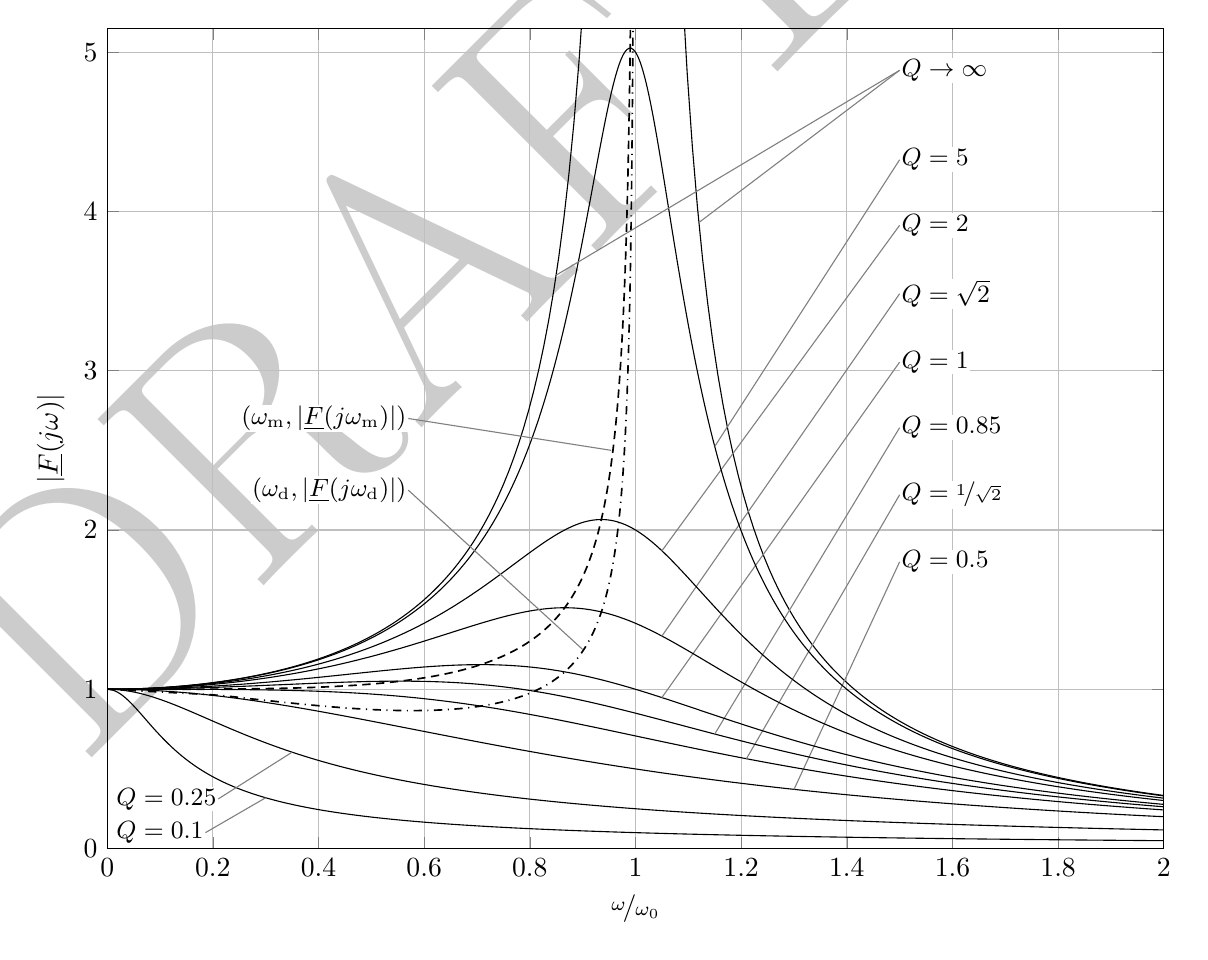
\begin{tikzpicture}
    \begin{axis}[ xlabel=$\nicefrac{\omega}{\omega_0}$
                , xmin=0
                , xmax=2
                , ymin=0
                , ymax=5.15
                , ylabel=$\left|\underline{F}(j\omega)\right|$
                , grid=major
                , ytick={0,1,...,5}
                , height=12cm
                , width=15cm
                ]

      \addplot [  draw=black
                , domain=0:0.95
                , samples=101
                ]
                {1/sqrt((1-x^2)^2)};

      \addplot [  draw=black
                , domain=1.03:2
                , samples=101
                ]
                {1/sqrt((1-x^2)^2)};

      \addplot [  draw=black
                , domain=0.71:5.5
                , samples=501
                , smooth
                , densely dashed
                , semithick
                ]
                ({sqrt(1-1/2/x^2)},{2*x^2/sqrt(4*x^2-1)});

      \addplot [  draw=black
                , domain=0.5:5.5
                , samples=501
                , smooth
                , dash dot
                , semithick
                ]
                ({sqrt(1-1/4/x^2)},{4*x^2/sqrt(16*x^2-3)});

      %Q=0.1
      \addplot [  draw=black
                , domain=0:2
                , samples=501
                , smooth
                ]
                {1/sqrt((1-x^2)^2+x^2/0.1^2)};

    \node[font=\small,fill=white,inner sep=0.5pt] (q01) 
      at (axis cs:0.1,0.1) {$Q=0.1$};
    \draw[thin,gray] (q01.east) -- (axis cs:0.3,0.319);

      %Q=0.25
      \addplot [  draw=black
                , domain=0:2
                , samples=501
                , smooth
                ]
                {1/sqrt((1-x^2)^2+x^2/0.25^2)};

    \node[font=\small,fill=white,inner sep=0.5pt,anchor=south west] (q025) 
      at ($(q01.north west) + (0,0.05)$) {$Q=0.25$};
    \draw[thin,gray] (q025.east) -- (axis cs:0.35,0.605);

      %Q=0.5
      \addplot [  draw=black
                , domain=0:2
                , samples=501
                , smooth
                ]
                {1/sqrt((1-x^2)^2+x^2/0.5^2)};
    \node[font=\small,fill=white,inner sep=0.5pt,anchor=west] (q05) 
      at (axis cs:1.5,1.8) {$Q=0.5$};
    \draw[thin,gray] (q05.west) -- (axis cs:1.3,0.371);

      %Q=1/sqrt(2)
      \addplot [  draw=black
                , domain=0:2
                , samples=501
                , smooth
                ]
                {1/sqrt((1-x^2)^2+x^2*2)};

    \node[font=\small,fill=white,inner sep=0.5pt,anchor=south west] (q0707) 
      at ($(q05.north west) + (0,0.25)$) {$Q=\nicefrac{1}{\sqrt{2}}$};
    \draw[thin,gray] (q0707.west) -- (axis cs:1.21,0.564);

      %Q=0.85
      \addplot [  draw=black
                , domain=0:2
                , samples=501
                , smooth
                ]
                {1/sqrt((1-x^2)^2+x^2/0.85^2)};

    \node[font=\small,fill=white,inner sep=0.5pt,anchor=south west] (q085) 
      at ($(q0707.north west) + (0,0.25)$) {$Q=0.85$};
    \draw[thin,gray] (q085.west) -- (axis cs:1.15,0.719);

       %Q=1
      \addplot [  draw=black
                , domain=0:2.5
                , samples=501
                , smooth
                ]
                {1/sqrt((1-x^2)^2+x^2/1^2)};

    \node[font=\small,fill=white,inner sep=0.5pt,anchor=south west] (q1) 
      at ($(q085.north west) + (0,0.25)$) {$Q=1$};
    \draw[thin,gray] (q1.west) -- (axis cs:1.05,0.948);

       %Q=sqrt(2)
      \addplot [  draw=black
                , domain=0:2.5
                , samples=501
                , smooth
                ]
                {1/sqrt((1-x^2)^2+x^2/2)};

    \node[font=\small,fill=white,inner sep=0.5pt,anchor=south west] (q141) 
      at ($(q1.north west) + (0,0.25)$) {$Q=\sqrt{2}$};
    \draw[thin,gray] (q141.west) -- (axis cs:1.05,1.334);

       %Q=2
      \addplot [  draw=black
                , domain=0:2
                , samples=501
                , smooth
                ]
                {1/sqrt((1-x^2)^2+x^2/2^2)};

    \node[font=\small,fill=white,inner sep=0.5pt,anchor=south west] (q2) 
      at ($(q141.north west) + (0,0.25)$) {$Q=2$};
    \draw[thin,gray] (q2.west) -- (axis cs:1.05,1.869);

      %Q=5
      \addplot [  draw=black
                , domain=0:2
                , samples=501
                , smooth
                ]
                {1/sqrt((1-x^2)^2+x^2/5^2)};

    \node[font=\small,fill=white,inner sep=0.5pt,anchor=south west] (q5) 
      at ($(q2.north west) + (0,0.25)$) {$Q=5$};
    \draw[thin,gray] (q5.west) -- (axis cs:1.15,2.524);

    \node[font=\small,fill=white,inner sep=0.5pt,anchor=south west] (qinfty) 
      at ($(q5.north west) + (0,0.4)$) {$Q \rightarrow \infty$};
    \draw[thin,gray] (qinfty.west) -- (axis cs:1.12,3.93);
    \draw[thin,gray] (qinfty.west) -- (axis cs:0.85,3.6);

    \node[font=\small,fill=white,inner sep=0.5pt,anchor=east] (wm) 
      at (axis cs: 0.57,2.7) 
      {$(\omega_{\mathrm{m}}, \left|\underline{F}(j\omega_{\mathrm{m}})\right|)$};
    \draw[thin,gray] (wm.east) -- (axis cs:0.954,2.5);

    \node[font=\small,fill=white,inner sep=0.5pt,anchor=east] (wr) 
      at (axis cs: 0.57,2.25) 
      {$(\omega_{\mathrm{d}}, \left|\underline{F}(j\omega_{\mathrm{d}})\right|)$};
    \draw[thin,gray] (wr.east) -- (axis cs:0.9,1.25);
    \end{axis}
  \end{tikzpicture}
  \caption{Magnitude of steady-state solution 
    $\left|\underline{F}(j\omega)\right|$ vs. normalized 
    frequency $\nicefrac{\omega}{\omega_0}$ for different qualities $Q$ and loci 
    of $(\omega_{\mathrm{m}}, \left|\underline{F}(j\omega_{\mathrm{m}})\right|)$
    and $(\omega_{\mathrm{r}}, \left|\underline{F}(j\omega_{\mathrm{r}})\right|)$}
  \label{fig:plot-fs}
\end{figure}

$\left|\underline{F}(s)\right|$ has a maximum at 
\begin{equation}
\omega_{\mathrm{m}}=
\begin{cases}
0 & \mathrm{when} \ Q <\frac{1}{\sqrt{2}} \\
\omega_0 \sqrt{1-\frac{1}{2Q^2}} & \mathrm{when} \ Q\geq\frac{1}{\sqrt{2}} \\
\end{cases} 
\end{equation}
and
\begin{equation}
\left|\underline{F}(j\omega_{\mathrm{m}})\right| =
\begin{cases}
1 & \mathrm{when} \ Q <\frac{1}{\sqrt{2}} \\
\frac{2 Q^2}{\sqrt{4Q^2-1}} & \mathrm{when} \ Q\geq\frac{1}{\sqrt{2}}. \\
\end{cases} 
\end{equation}
It is obvious that  $\omega_{\mathrm{m}} \rightarrow \omega_{\mathrm{0}}$
for $Q \rightarrow \infty$ and therefore 
$\left|\underline{F}(j\omega_{\mathrm{m}})\right| \rightarrow  Q$
for $Q \rightarrow \infty$.
The locus $(\omega_{\mathrm{m}}, \left|\underline{F}(j\omega_{\mathrm{m}})\right|)$
is shown in Fig.~\ref{fig:plot-fs} (dashed line).
We refer to $\omega_{\mathrm{m}}$ when $Q\geq\nicefrac{1}{\sqrt{2}}$%
\footnote{The case $Q = \nicefrac{1}{\sqrt{2}}$  results
in a Butterworth filter response 
(conf. subsection \ref{subsec:examples:butterworth}).}
as resonant frequent $\omega_{\mathrm{r}}$.

\medskip

The poles of $\underline{F}(s)$ are
\begin{equation}\label{eq:poles}
p_{1,2} = - \zeta \omega_0 \pm \omega_0 \sqrt{\zeta^2-1} = - \alpha \pm \omega_0 \sqrt{\zeta^2-1}.
\end{equation}

\medskip

For $0<\zeta < 1$ (conf. column \textit{Underdamped} in Tab. \ref{tab:pz}), 
we transform \eqref{eq:poles} to
\begin{equation}\label{eq:poles-underdamped}
p_{1,2} = - \alpha \pm j \omega_{\mathrm{d}},
\end{equation}
with the damped oscillating frequency 
\begin{equation}\label{eq:poles}
\omega_{\mathrm{d}} = \omega_0 \sqrt{1-\zeta^2} = \omega_0 \sqrt{1-\frac{1}{4 Q^2}}
\end{equation}
and
\begin{equation}
\left|\underline{F}(j\omega_{\mathrm{d}})\right| = \frac{4 Q^2}{\sqrt{16 Q^2 -3}}.
\end{equation}

Tab.~\ref{tab:char-fs} summarizes some interesting values of
$\underline{F}(j\omega)$.
\begin{table}[H]
\centering
\caption{Characteristics of steady-state solution 
  $\left|\underline{F}(j\omega)\right|$ for different $Q$}
\begin{tabular}{cccccc}
\toprule
$Q$                      & $\zeta$                   & $\nicefrac{\omega_{\mathrm{r}}}{\omega_0}$ & $\left|\nicefrac{\underline{F}(\omega_{\mathrm{r}})}{\underline{F}(\omega_{\mathrm{0}})}\right|$ & $\nicefrac{\omega_{\mathrm{d}}}{\omega_0}$ & $\left|\nicefrac{\underline{F}(\omega_{\mathrm{d}})}{\underline{F}(\omega_{\mathrm{0}})}\right|$ \\ \midrule
0.1                      & 5                         & -                                          & -                                                                                                & -                                          & -                                                                                                \\
0.25                     & 2                         & -                                          & -                                                                                                & -                                          & -                                                                                                \\ 
0.5                      & 1                         & -                                          & -                                                                                                & 0                                          & 2                                                                                                \\
$\nicefrac{1}{\sqrt{3}}$ & $\nicefrac{\sqrt{3}}{2}$  & -                                          & -                                                                                                & 0.5                                        & 1.512                                                                                            \\ 
$\nicefrac{1}{\sqrt{2}}$ & $\nicefrac{1}{\sqrt{2}}$  & 0                                          & $\sqrt{2}$                                                                                       & $\nicefrac{1}{\sqrt{2}}$                   & 1.265                                                                                            \\
0.85                     & 0.588                     & 0.555                                      & 1.237                                                                                            & 0.809                                      & 1.162                                                                                            \\  
1                        & 0.5                       & $\nicefrac{1}{\sqrt{2}}$                   & 1.155                                                                                            & $\nicefrac{\sqrt{3}}{2}$                   & 1.109                                                                                            \\  
$\sqrt{2}$               & 0.354                     & $\nicefrac{\sqrt{3}}{2}$                   & 1.069                                                                                            & 0.935                                      & 1.05                                                                                             \\
2                        & 0.25                      & 0.935                                      & 1.033                                                                                            & 0.968                                      & 1.024                                                                                            \\ 
5                        & 0.1                       & 0.99                                       & 1.005                                                                                            & 0.995                                      & 1.004                                                                                            \\ 
$\infty$                 & 0                         & 1                                          & 1                                                                                                & 1                                          & 1                                                                                                \\ \toprule
\end{tabular}
\label{tab:char-fs}
\end{table}

The phase of $\underline{F}(j\omega)$ is
\begin{equation}
\arg\left(\underline{F}(j\omega)\right)= 
  -\atan\left(\frac{\frac{\omega}{Q \omega_0}}
                   {1-\left(\frac{\omega}{\omega_0}\right)^2}\right).
\end{equation}
A plot of the phase for different $Q$ is provided in Fig. \ref{fig:plot-fs-arg}.
All curves cross the point already discovered in
\eqref{eq:argf0}.
\begin{figure}[H]
  \centering
  \begin{tikzpicture}
    \begin{axis}[ xlabel=$\nicefrac{\omega}{\omega_0}$
                , xmin=0
                , xmax=2
                , ymin=-180
                , ymax=0
                , ylabel=$\arg\left(\underline{F}(j\omega)\right)$ in \si{\degree}
                , grid=major
                , ytick={0,-45,-90,...,-180}
                , height=8cm
                , width=15cm
                ]

    \addplot[ semithick
            ]
            table
            [ x=w
            , y=q01
            , col sep=comma
            ] {phase.csv};
    \node[font=\small,anchor=east,inner sep=0.5pt] 
      (q01) at (axis cs:0.5,-95) {$Q=0.1$};
    \draw[thin,gray] (q01.east) -- (0.552,-82.82);

    \addplot[ semithick
            ]
            table
            [ x=w
            , y=q025
            , col sep=comma
            ] {phase.csv};
    \node[font=\small,anchor=east,inner sep=0.5pt] 
      (q025) at (axis cs:0.5,-105) {$Q=0.25$};
    \draw[thin,gray] (q025.east) -- (0.592,-74.66);

    \addplot[ semithick
            ]
            table
            [ x=w
            , y=q05
            , col sep=comma
            ] {phase.csv};
    \addplot[ semithick
            ]
            table
            [ x=w
            , y=q025
            , col sep=comma
            ] {phase.csv};
    \node[font=\small,anchor=east,inner sep=0.5pt] 
      (q05) at (axis cs:0.5,-115) {$Q=0.5$};
    \draw[thin,gray] (q05.east) -- (0.66,-66.85);

    \addplot[ semithick
            ]
            table
            [ x=w
            , y=q1oversqrt3
            , col sep=comma
            ] {phase.csv};
    \node[font=\small,anchor=east,inner sep=0.5pt] 
      (q1oversqrt3) at (axis cs:0.5,-125) {$Q=\nicefrac{1}{\sqrt{3}}$};
    \draw[thin,gray] (q1oversqrt3.east) -- (0.708,-67.87);

    \addplot[ semithick
            ]
            table
            [ x=w
            , y=q1oversqrt2
            , col sep=comma
            ] {phase.csv};
    \node[font=\small,anchor=east,inner sep=0.5pt] 
      (q1oversqrt2) at (axis cs:0.5,-135) {$Q=\nicefrac{1}{\sqrt{2}}$};
    \draw[thin,gray] (q1oversqrt2.east) -- (0.792,-71.59);

    \addplot[ semithick
            ]
            table
            [ x=w
            , y=q085
            , col sep=comma
            ] {phase.csv};
    \node[font=\small,anchor=west,inner sep=0.5pt] 
      (q085) at (axis cs:1,-55) {$Q=0.85$};
    \draw[thin,gray] (q085.west) -- (0.832,-72.55);

    \addplot[ semithick
            ]
            table
            [ x=w
            , y=q1
            , col sep=comma
            ] {phase.csv};   
    \node[font=\small,anchor=west,inner sep=0.5pt] 
      (q1) at (axis cs:1,-45) {$Q=1$};
    \draw[thin,gray] (q1.west) -- (0.832,-69.70);
            
    \addplot[ semithick
            ]
            table
            [ x=w
            , y=qsqrt2
            , col sep=comma
            ] {phase.csv};   
    \node[font=\small,anchor=west,inner sep=0.5pt] 
      (qsqrt2) at (axis cs:1,-35) {$Q=\sqrt{2}$};
    \draw[thin,gray] (qsqrt2.west) -- (0.832,-62.38);

    \addplot[ semithick
            ]
            table
            [ x=w
            , y=q2
            , col sep=comma
            ] {phase.csv};
    \node[font=\small,anchor=west,inner sep=0.5pt] 
      (q2) at (axis cs:1,-25) {$Q=2$};
    \draw[thin,gray] (q2.west) -- (0.832,-53.50);

    \addplot[ semithick
            ]
            table
            [ x=w
            , y=q5
            , col sep=comma
            ] {phase.csv};     
    \node[font=\small,anchor=west,inner sep=0.5pt] 
      (q5) at (axis cs:1,-15) {$Q=5$};
    \draw[thin,gray] (q5.west) -- (0.832,-28.40);

    \end{axis}
  \end{tikzpicture}
  \caption{Phase of steady-state solution $\arg\left(\underline{F}(j\omega)\right)$}
  \label{fig:plot-fs-arg}
\end{figure}

The group delay is

\begin{equation}
\tau_{\mathrm{g}} = -\frac{\mathrm{d} \arg\left(\underline{F}(j\omega)\right)}{\mathrm{d}\omega}
                  = \frac{Q}{\omega_0} \frac{1+\left(\frac{\omega}{\omega_0}\right)^2}{Q^2 + \left(1-2Q^2\right) \left(\frac{\omega}{\omega_0}\right)^2 + Q^2 \left(\frac{\omega}{\omega_0}\right)^4}.
\end{equation}

\section{Poles}

Depending on $Q$, we can define four different cases. 
They are depicted in Tab.~\ref{tab:pz}.

\begin{table}[H]
  \centering
  \caption{Poles of $\underline{F}(s)$}
  \begin{tabular}{ccccc}
  \toprule
                           & \textbf{Overdamped}               & \textbf{Critically damped} & \textbf{Underdamped}                    & \textbf{Undamped}     \\ \midrule
  $Q$                       & $\left(0, \nicefrac{1}{2}\right)$ & $\nicefrac{1}{2}$          & $\left(\nicefrac{1}{2}, \infty\right)$ & $\rightarrow \infty$  \\ 
  $\zeta$                   & $\left(1, \infty\right)$          & $1$                        & $\left(0, 1\right)$                    & $0$                   \\ \hline
  $p_{1,2}$                 & $\neq$                            & $=$                        & complex conj.                          & complex conj.         \\
  $\Re\left(p_{1,2}\right)$ & $<0$                              & $<0$                       & $<0$                                   & $=0$                  \\
  $\Im\left(p_{1,2}\right)$ & $=0$                              & $=0$                       & $\neq0$                                & $\neq0$               \\
  Plot                      & \ref{fig:pz:overdamped}           & \ref{fig:pz:critdamped}    & \ref{fig:pz:underdamped}               & \ref{fig:pz:undamped} \\ \toprule
  \end{tabular}
  \label{tab:pz}
\end{table}

\begin{figure}[H]
  \centering
  \begin{subfigure}[b]{0.475\textwidth}
    \centering
    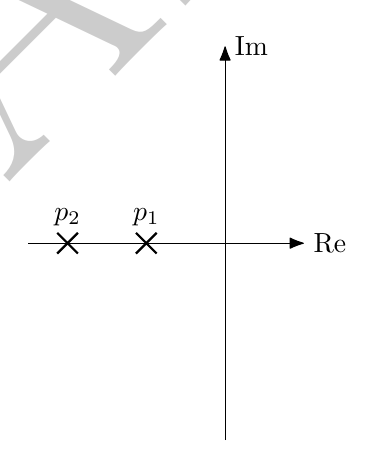
\begin{tikzpicture}[scale=1.0]
      \draw[-{Latex[round,scale=1.2,round]}] (-2.5,0) -- (1,0);
      \node[anchor=west] at (1,0) {Re};
      \draw[-{Latex[round,scale=1.2,round]}] (0,-2.5) -- (0,2.5);
      \node[anchor=west] at (0,2.5) {Im};

      \node[cross out,draw=black,thick] at (-2, 0) {};
      \node[cross out,draw=black,thick] at (-1, 0) {};
      \node[anchor=south] at (-2, 0.1) {$p_2$};
      \node[anchor=south] at (-1, 0.1) {$p_1$};
    \end{tikzpicture}
    \caption{Overdamped}
    \label{fig:pz:overdamped}
  \end{subfigure}%
  \hfill
  \begin{subfigure}[b]{0.475\textwidth}
    \centering
    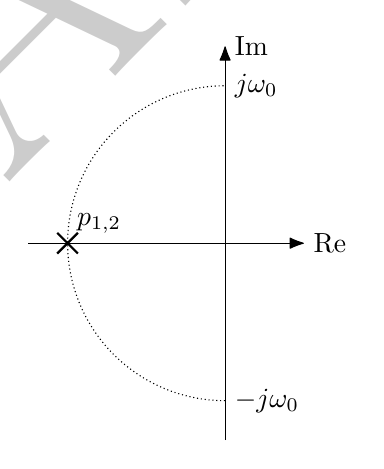
\begin{tikzpicture}[scale=1.0]
      \draw[densely dotted] plot[smooth,domain=180:360, samples=501] 
        ({2*sin(\x)},{2*cos(\x)});
      \draw[-{Latex[round,scale=1.2,round]}] (-2.5,0) -- (1,0);
      \node[anchor=west] at (1,0) {Re};
      \draw[-{Latex[round,scale=1.2,round]}] (0,-2.5) -- (0,2.5);
      \node[anchor=west] at (0,2.5) {Im};
      \node[anchor=west] at (0, 2) {$ j \omega_0$};
      \node[anchor=west] at (0,-2) {$-j \omega_0$};

      \node[cross out,draw=black,thick] at (-2, 0) {};
      \node[anchor=south] at (-1.6, 0) {$p_{1,2}$};
    \end{tikzpicture}
    \caption{Critically damped}
    \label{fig:pz:critdamped}
  \end{subfigure}
  \vskip\baselineskip
  \begin{subfigure}[b]{0.475\textwidth}
    \centering
    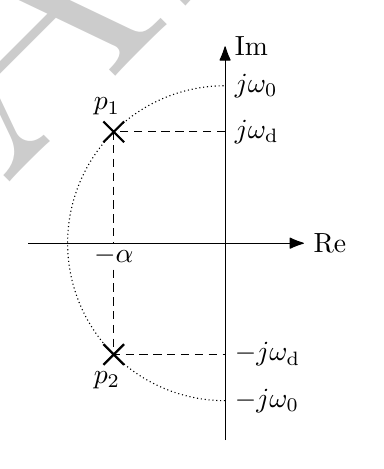
\begin{tikzpicture}[scale=1.0]
      \draw[densely dotted] plot[smooth,domain=180:360, samples=501] 
        ({2*sin(\x)},{2*cos(\x)});

      \draw[-{Latex[round,scale=1.2,round]}] (-2.5,0) -- (1,0);
      \node[anchor=west] at (1,0) {Re};
      \draw[-{Latex[round,scale=1.2,round]}] (0,-2.5) -- (0,2.5);
      \node[anchor=west] at (0,2.5) {Im};

      \node[cross out,draw=black,thick] at (-1.414,  1.414) {};
      \node[cross out,draw=black,thick] at (-1.414, -1.414) {};
      \node[anchor=south] at (-1.5, 1.5) {$p_1$};
      \node[anchor=north] at (-1.5,-1.5) {$p_2$};

      \draw[densely dashed] (0, 1.414) -- (-1.414, 1.414) -- 
                            (-1.414, -1.414) -- (0, -1.414);

      \node[anchor=west] at (0, 2) {$ j \omega_0$};
      \node[anchor=west] at (0,-2) {$-j \omega_0$};

      \node[anchor=west] at (0, 1.414) {$ j \omega_{\mathrm{d}}$};
      \node[anchor=west] at (0,-1.414) {$-j \omega_{\mathrm{d}}$};

      \node[anchor=north,fill=white,inner sep=1pt] at (-1.414,0) {$-\alpha$};
    \end{tikzpicture}
    \caption{Underdamped}
    \label{fig:pz:underdamped}
  \end{subfigure}%
  \hfill
  \begin{subfigure}[b]{0.475\textwidth}
    \centering
    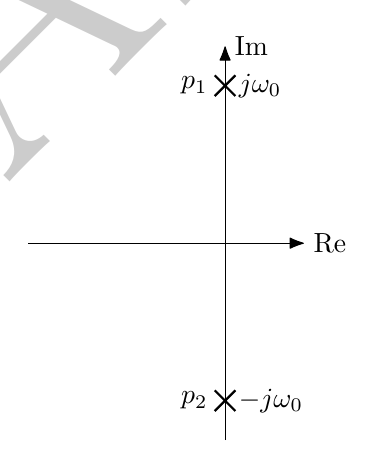
\begin{tikzpicture}[scale=1.0]
      \draw[-{Latex[round,scale=1.2,round]}] (-2.5,0) -- (1,0);
      \node[anchor=west] at (1,0) {Re};
      \draw[-{Latex[round,scale=1.2,round]}] (0,-2.5) -- (0,2.5);
      \node[anchor=west] at (0,2.5) {Im};

      \node[cross out,draw=black,thick] at (0,  2) {};
      \node[cross out,draw=black,thick] at (0, -2) {};
      \node[anchor=east] at (-0.1, 2) {$p_1$};
      \node[anchor=east] at (-0.1,-2) {$p_2$};

      \node[anchor=west] at (0.05, 2) {$ j \omega_0$};
      \node[anchor=west] at (0.05,-2) {$-j \omega_0$};
    \end{tikzpicture}
    \caption{Undamped}
    \label{fig:pz:undamped}
  \end{subfigure}
  \caption{Pole-zero plot}
  \label{fig:squarelawtransf}
\end{figure}


\section{Step Response}

Next, we will calculate the step response, i.e. $y(t)$ for the input signal
\begin{equation}
x(t) =
\begin{cases}
0 & \mathrm{when} \ t < 0    \\
1 & \mathrm{when} \ t \geq 0 \\
\end{cases}.
\end{equation}

First, we need to introduce the abbreviations
\begin{equation}
 T_0 = \frac{2\pi}{\omega_0}
\end{equation}
and
\begin{equation}\label{eq:td}
 T_{\mathrm{d}} = \frac{2\pi}{\omega_{\mathrm{d}}} 
                = \frac{2\pi}{\omega_0 \sqrt{1-\zeta^2}}
                = \frac{T_0}{\sqrt{1-\zeta^2}} 
                = \frac{T_0}{\sqrt{1-\frac{1}{4 Q^2}}}.
\end{equation}

Using \cite{golnaraghi-acs-10}, we can derive 
\begin{equation}
y(t)=
\begin{cases}
1-\left(\frac{p_2}{p_2-p_1} e^{p_1 t}-\frac{p_1}{p_2-p_1} e^{p_2 t}\right)             & \mathrm{when} \ Q <\frac{1}{2} \\
1 - e^{-\omega_0 t} (1+\omega_0 t)                                                     & \mathrm{when} \ Q = \frac{1}{2} \\
1-\frac{e^{-\alpha t}}{\sin(\phi)} \cdot \sin\left(\omega_{\mathrm{d}} t + \phi\right) & \mathrm{when} \ \frac{1}{2} < Q  \\
1 - \cos(\omega_0 t)                                                                   & \mathrm{when} \ Q \rightarrow \infty \\
\end{cases}, 
\end{equation}
with
\begin{equation}
\zeta = \cos(\phi).
\end{equation}

The output signal $y(t)$ is shown in Fig. \ref{fig:step-response}
for different $Q$.
\begin{figure}[H]
  \centering
  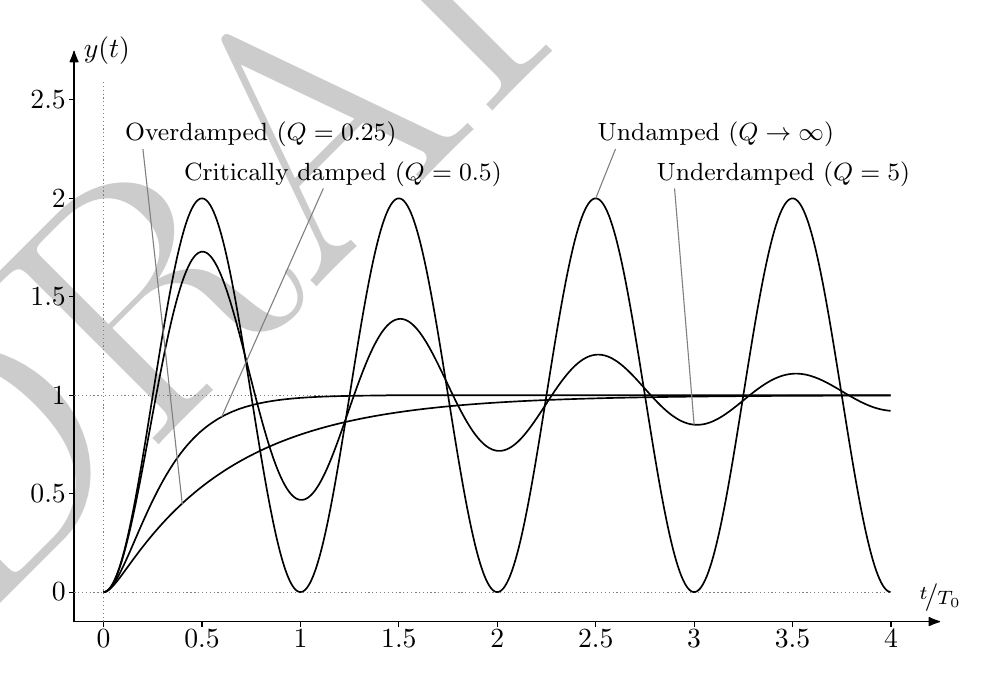
\begin{tikzpicture}[scale=2.5]

    \draw[{Latex[round,scale=1.0,round]}-{Latex[round,scale=1.0,round]}] 
      (-0.15,2.75) -- (-0.15,-0.15) -- (4.25,-0.15);

    \node[anchor=south] at  (4.25,-0.15) {$\nicefrac{t}{T_0}$}; 
    \node[anchor=west]  at  (-0.15,2.75) {$y(t)$}; 

    \draw (0.0,-0.15) --++ (0,-0.025) node[anchor=north, inner sep=1pt] {0};
    \draw (0.5,-0.15) --++ (0,-0.025) node[anchor=north, inner sep=1pt] {0.5};
    \draw (1.0,-0.15) --++ (0,-0.025) node[anchor=north, inner sep=1pt] {1};
    \draw (1.5,-0.15) --++ (0,-0.025) node[anchor=north, inner sep=1pt] {1.5};
    \draw (2.0,-0.15) --++ (0,-0.025) node[anchor=north, inner sep=1pt] {2};
    \draw (2.5,-0.15) --++ (0,-0.025) node[anchor=north, inner sep=1pt] {2.5};
    \draw (3.0,-0.15) --++ (0,-0.025) node[anchor=north, inner sep=1pt] {3};
    \draw (3.5,-0.15) --++ (0,-0.025) node[anchor=north, inner sep=1pt] {3.5};
    \draw (4.0,-0.15) --++ (0,-0.025) node[anchor=north, inner sep=1pt] {4};

    \draw (-0.15,0.0) --++ (-0.025,0) node[anchor=east, inner sep=1pt] {0};
    \draw (-0.15,0.5) --++ (-0.025,0) node[anchor=east, inner sep=1pt] {0.5};
    \draw (-0.15,1.0) --++ (-0.025,0) node[anchor=east, inner sep=1pt] {1};
    \draw (-0.15,1.5) --++ (-0.025,0) node[anchor=east, inner sep=1pt] {1.5};
    \draw (-0.15,2.0) --++ (-0.025,0) node[anchor=east, inner sep=1pt] {2};
    \draw (-0.15,2.5) --++ (-0.025,0) node[anchor=east, inner sep=1pt] {2.5};

    \draw[densely dotted,gray] plot[smooth,domain=-0.15:4, samples=2] 
      ({\x},{1});
    \draw[densely dotted,gray] plot[smooth,domain=-0.15:4, samples=2] 
      ({\x},{0});
    \draw[densely dotted,gray] plot[smooth,domain=-0.15:2.6, samples=2] 
      ({0},{\x});

    \draw[semithick] plot[smooth,domain=0:4, samples=501] 
      ({\x},{1-((-2+sqrt(3))/(2*sqrt(3))*e^(2*pi*(-2-sqrt(3))*\x)-(-2-sqrt(3))/(2*sqrt(3))*e^(2*pi*(-2+sqrt(3))*\x))});

    \draw[semithick] plot[smooth,domain=0:4, samples=501] 
      ({\x},{1-e^(-2*pi*\x)*(1+2*pi*\x)});

    \draw[semithick] plot[smooth,domain=0:4, samples=501] 
      ({\x},{1-e^(-0.1*2*pi*\x)*sin(360*sqrt(1-0.1^2)*\x+acos(0.1))/sin(acos(0.1))});

    \draw[semithick] plot[smooth,domain=0:4, samples=501] 
     ({\x},{1-cos(360*\x)});

    \node[font=\small,anchor=south west,inner sep=0.5pt] 
      (od) at (0.4,2.05) {Critically damped ($Q=0.5$)};
    \node[font=\small,anchor=south west,inner sep=0.5pt] 
      (cd) at (0.1,2.25) {Overdamped ($Q=0.25$)};
    \node[font=\small,anchor=south west,inner sep=0.5pt] 
      (ud) at (2.5,2.25) {Undamped ($Q \rightarrow \infty$)};
    \node[font=\small,anchor=south west,inner sep=0.5pt] 
      (und) at (2.8,2.05) {Underdamped ($Q=5$)};

    \draw[thin,gray] ($(cd.south west) + (0.1,0)$) -- (0.4,0.445);
    \draw[thin,gray] ($(od.south) + (-0.1,0)$) -- (0.6,0.89);
    \draw[thin,gray] ($(ud.south west) + (0.1,0)$) -- (2.5,2);
    \draw[thin,gray] ($(und.south west) + (0.1,0)$) -- (3,0.85);
  \end{tikzpicture}
  \caption{Step response for different $Q$}
  \label{fig:step-response}
\end{figure}

\begin{itemize}
  \item $y(t) \rightarrow 1$ for $t \rightarrow \infty$ when $Q < \infty$.
  \item $y(t) > 1$ and oscillates only for $Q > 0.5$. 
  \item The period in the \textit{underdamped} case is higher than in the 
    \textit{undamped} case (conf. \eqref{eq:td}).
\end{itemize}

The functions $1 \pm \exp\left\{-\alpha t\right\}$ are an envelope
for $y(t)$ in the \textit{underdamped} case (Fig. \ref{fig:step-response-env}).
\begin{figure}[H]
  \centering
  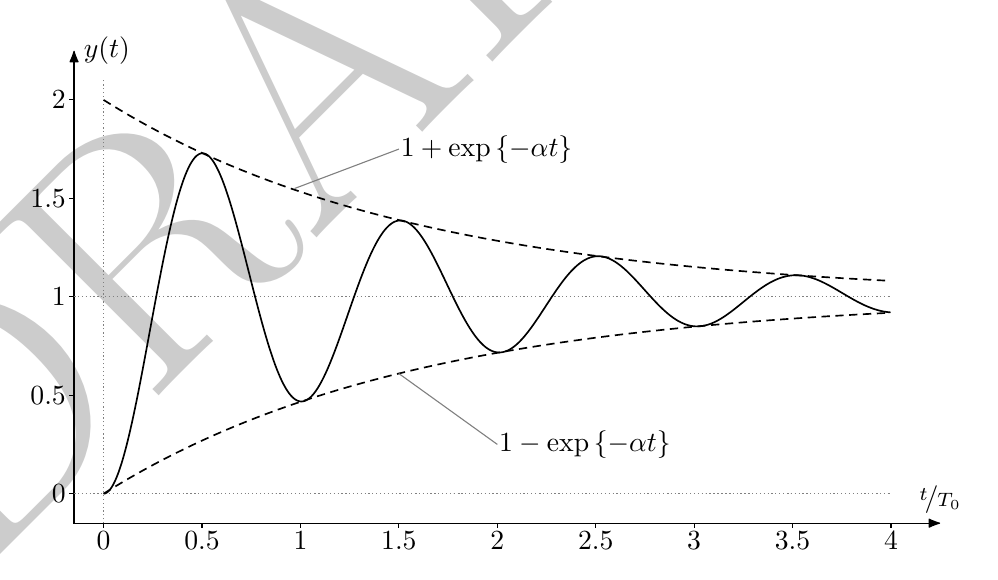
\begin{tikzpicture}[scale=2.5]

    \draw[{Latex[round,scale=1.0,round]}-{Latex[round,scale=1.0,round]}] 
      (-0.15,2.25) -- (-0.15,-0.15) -- (4.25,-0.15);

    \node[anchor=south] at  (4.25,-0.15) {$\nicefrac{t}{T_0}$}; 
    \node[anchor=west]  at  (-0.15,2.25) {$y(t)$}; 

    \draw (0.0,-0.15) --++ (0,-0.025) node[anchor=north, inner sep=1pt] {0};
    \draw (0.5,-0.15) --++ (0,-0.025) node[anchor=north, inner sep=1pt] {0.5};
    \draw (1.0,-0.15) --++ (0,-0.025) node[anchor=north, inner sep=1pt] {1};
    \draw (1.5,-0.15) --++ (0,-0.025) node[anchor=north, inner sep=1pt] {1.5};
    \draw (2.0,-0.15) --++ (0,-0.025) node[anchor=north, inner sep=1pt] {2};
    \draw (2.5,-0.15) --++ (0,-0.025) node[anchor=north, inner sep=1pt] {2.5};
    \draw (3.0,-0.15) --++ (0,-0.025) node[anchor=north, inner sep=1pt] {3};
    \draw (3.5,-0.15) --++ (0,-0.025) node[anchor=north, inner sep=1pt] {3.5};
    \draw (4.0,-0.15) --++ (0,-0.025) node[anchor=north, inner sep=1pt] {4};

    \draw (-0.15,0.0) --++ (-0.025,0) node[anchor=east, inner sep=1pt] {0};
    \draw (-0.15,0.5) --++ (-0.025,0) node[anchor=east, inner sep=1pt] {0.5};
    \draw (-0.15,1.0) --++ (-0.025,0) node[anchor=east, inner sep=1pt] {1};
    \draw (-0.15,1.5) --++ (-0.025,0) node[anchor=east, inner sep=1pt] {1.5};
    \draw (-0.15,2.0) --++ (-0.025,0) node[anchor=east, inner sep=1pt] {2};

    \draw[densely dotted,gray] plot[smooth,domain=-0.15:4, samples=2] 
      ({\x},{1});
    \draw[densely dotted,gray] plot[smooth,domain=-0.15:4, samples=2] 
      ({\x},{0});
    \draw[densely dotted,gray] plot[smooth,domain=-0.15:2.1, samples=2] 
      ({0},{\x});

    \draw[semithick] plot[smooth,domain=0:4, samples=501] 
      ({\x},{1-e^(-0.1*2*pi*\x)*sin(360*sqrt(1-0.1^2)*\x+acos(0.1))/sin(acos(0.1))});

    \draw [semithick,densely dashed] plot
          [ 
          , domain=0:4
          , samples=501
          , smooth
          ] ({\x},{1+exp(-0.1*2*pi*\x)});
    \draw [semithick,densely dashed] plot
          [ 
          , domain=0:4
          , samples=501
          , smooth
          ] ({\x},{1-exp(-0.1*2*pi*\x)});

    \node[anchor=west,inner sep=0.5pt] (t) 
      at (1.5,1.75) {$1+\exp\left\{-\alpha t\right\}$}; 
    \node[anchor=west,inner sep=0.5pt] (b) 
      at (2.0,0.25) {$1-\exp\left\{-\alpha t\right\}$};   

    \draw[thin,gray] (t.west) -- (0.97,1.55);  
    \draw[thin,gray] (b.west) -- (1.5,0.61);  
  \end{tikzpicture}
  \caption{Underdamped step response for $Q=5$ including evelopes}
  \label{fig:step-response-env}
\end{figure}

Fig. \ref{fig:step-response-ud} shows the step response for
different $Q>0.5$ (\textit{Underdamped}).
\begin{figure}[H]
  \centering
  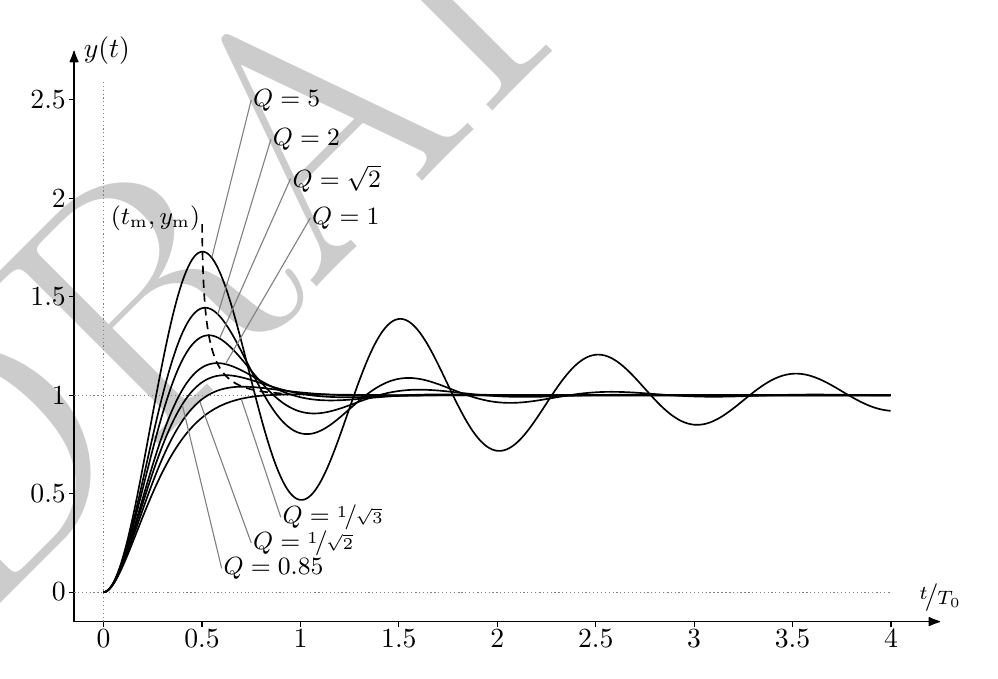
\begin{tikzpicture}[scale=2.5]

    \draw[{Latex[round,scale=1.0,round]}-{Latex[round,scale=1.0,round]}] 
      (-0.15,2.75) -- (-0.15,-0.15) -- (4.25,-0.15);

    \node[anchor=south] at  (4.25,-0.15) {$\nicefrac{t}{T_0}$}; 
    \node[anchor=west]  at  (-0.15,2.75) {$y(t)$}; 

    \draw (0.0,-0.15) --++ (0,-0.025) node[anchor=north, inner sep=1pt] {0};
    \draw (0.5,-0.15) --++ (0,-0.025) node[anchor=north, inner sep=1pt] {0.5};
    \draw (1.0,-0.15) --++ (0,-0.025) node[anchor=north, inner sep=1pt] {1};
    \draw (1.5,-0.15) --++ (0,-0.025) node[anchor=north, inner sep=1pt] {1.5};
    \draw (2.0,-0.15) --++ (0,-0.025) node[anchor=north, inner sep=1pt] {2};
    \draw (2.5,-0.15) --++ (0,-0.025) node[anchor=north, inner sep=1pt] {2.5};
    \draw (3.0,-0.15) --++ (0,-0.025) node[anchor=north, inner sep=1pt] {3};
    \draw (3.5,-0.15) --++ (0,-0.025) node[anchor=north, inner sep=1pt] {3.5};
    \draw (4.0,-0.15) --++ (0,-0.025) node[anchor=north, inner sep=1pt] {4};

    \draw (-0.15,0.0) --++ (-0.025,0) node[anchor=east, inner sep=1pt] {0};
    \draw (-0.15,0.5) --++ (-0.025,0) node[anchor=east, inner sep=1pt] {0.5};
    \draw (-0.15,1.0) --++ (-0.025,0) node[anchor=east, inner sep=1pt] {1};
    \draw (-0.15,1.5) --++ (-0.025,0) node[anchor=east, inner sep=1pt] {1.5};
    \draw (-0.15,2.0) --++ (-0.025,0) node[anchor=east, inner sep=1pt] {2};
    \draw (-0.15,2.5) --++ (-0.025,0) node[anchor=east, inner sep=1pt] {2.5};

    \draw[densely dotted,gray] plot[smooth,domain=-0.15:4, samples=2] 
      ({\x},{1});
    \draw[densely dotted,gray] plot[smooth,domain=-0.15:4, samples=2] 
      ({\x},{0});
    \draw[densely dotted,gray] plot[smooth,domain=-0.15:2.6, samples=2] 
      ({0},{\x});

    \draw[semithick] plot[smooth,domain=0:4, samples=501] 
      ({\x},{1-e^(-0.1*2*pi*\x)*sin(360*sqrt(1-0.1^2)*\x+acos(0.1))/sin(acos(0.1))});

    \draw[semithick] plot[smooth,domain=0:4, samples=501] 
      ({\x},{1-e^(-0.25*2*pi*\x)*sin(360*sqrt(1-0.25^2)*\x+acos(0.25))/sin(acos(0.25))});

    \draw[semithick] plot[smooth,domain=0:4, samples=501] 
      ({\x},{1-e^(-0.354*2*pi*\x)*sin(360*sqrt(1-0.354^2)*\x+acos(0.354))/sin(acos(0.354))});

    \draw[semithick] plot[smooth,domain=0:4, samples=501] 
      ({\x},{1-e^(-0.5*2*pi*\x)*sin(360*sqrt(1-0.5^2)*\x+acos(0.5))/sin(acos(0.5))});      

    \draw[semithick] plot[smooth,domain=0:4, samples=501] 
      ({\x},{1-e^(-0.588*2*pi*\x)*sin(360*sqrt(1-0.588^2)*\x+acos(0.588))/sin(acos(0.588))});      

    \draw[semithick] plot[smooth,domain=0:4, samples=501] 
      ({\x},{1-e^(-0.707*2*pi*\x)*sin(360*sqrt(1-0.707^2)*\x+acos(0.707))/sin(acos(0.707))});  

    \draw[semithick] plot[smooth,domain=0:4, samples=501] 
      ({\x},{1-e^(-0.866*2*pi*\x)*sin(360*sqrt(1-0.866^2)*\x+acos(0.866))/sin(acos(0.866))});  

    \draw [semithick,densely dashed] plot
          [ 
          , domain=0.6:13
          , samples=501
          , smooth
          ] ({\x/sqrt(4*\x^2-1)},{1+exp(-pi/sqrt(4*\x^2-1))});

    \node[font=\small,anchor=east,inner sep=0.5pt] 
      (ok) at (0.5,1.9) {$(t_{\mathrm{m}},y_{\mathrm{m}})$}; 

    \node[font=\small,anchor=west,inner sep=0.5pt] (q5) at (0.75,2.5) {$Q=5$}; 
    \node[font=\small,anchor=west,inner sep=0.5pt] (q2) at (0.85,2.3) {$Q=2$}; 
    \node[font=\small,anchor=west,inner sep=0.5pt] (qsqrt2) at (0.95,2.1) {$Q=\sqrt{2}$}; 
    \node[font=\small,anchor=west,inner sep=0.5pt] (q1) at (1.05,1.9) {$Q=1$};
    \node[font=\small,anchor=west,inner sep=0.5pt] (qoversqrt3) at (0.9,0.38) {$Q=\nicefrac{1}{\sqrt{3}}$};
    \node[font=\small,anchor=west,inner sep=0.5pt] (qoversqrt2) at (0.75,0.25) {$Q=\nicefrac{1}{\sqrt{2}}$};
    \node[font=\small,anchor=west,inner sep=0.5pt] (q085) at (0.6,0.12) {$Q=0.85$};

    \draw[thin,gray] (q5.west) -- (0.55,1.7);
    \draw[thin,gray] (q2.west) -- (0.58,1.41);
    \draw[thin,gray] (qsqrt2.west) -- (0.59,1.29);   
    \draw[thin,gray] (q1.west) -- (0.62,1.16);  
    \draw[thin,gray] (qoversqrt3.west) -- (0.7,0.98); 
    \draw[thin,gray] (qoversqrt2.west) -- (0.49,0.965); 
    \draw[thin,gray] (q085.west) -- (0.4,0.95);     
  \end{tikzpicture}
  \caption{Underdamped step responses}
  \label{fig:step-response-ud}
\end{figure}

\subsection{Overshoot}

The waveform $y(t)$ has a maximum at 
\begin{equation}
t_{\mathrm{m}} = T_0 \frac{Q}{\sqrt{4Q^2-1}}
\end{equation}
for $Q > \nicefrac{1}{2}$ with
\begin{equation}
y(t_{\mathrm{m}}) =y_{\mathrm{m}} = 1 + \exp\left\{-\frac{\pi}{\sqrt{4Q^2-1}}\right\}.
\end{equation}
With that, we can calculate the overshoot
\begin{equation}
\mathrm{OS} =  \exp\left\{-\frac{\pi}{\sqrt{4Q^2-1}}\right\}.
\end{equation}
The higher the quality $Q$, the higher the overshoot.
In the \textit{undamped} case, the overshoot is \SI{100}{\percent}.
Conversely, we can directly calculate the quality 
\begin{equation}
Q = \left|\frac{\sqrt{\ln\left(\mathrm{OS}\right)^2+\pi^2}}{2\ln\left(\mathrm{OS}\right)}\right|
\end{equation}
based on the given overshoot.
Fig. \ref{fig:os1} and \ref{fig:os2} show the overshoot as 
a function of the quality $Q$.
\begin{figure}[H]
  \centering
  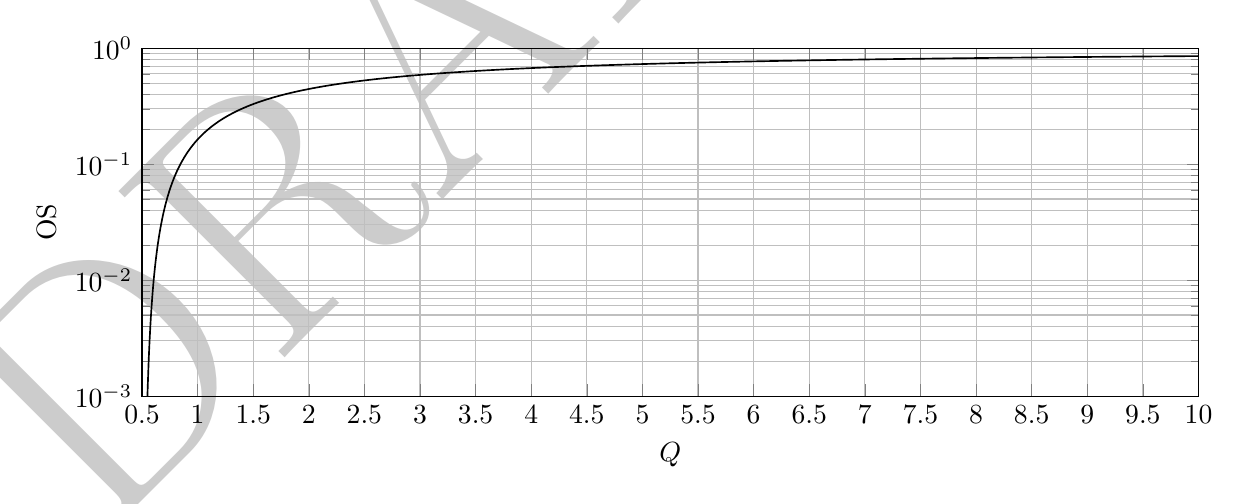
\begin{tikzpicture}
    \begin{axis}[ xlabel=$Q$ 
                , xmin=0.5
                , xmax=10
                , ymin=0.001
                , ymax=1
                , ylabel=$\mathrm{OS}$
                , grid=both
                , xtick={0.5,1,...,10}
                , ymode=log
                , width=15cm
                , height=6cm
                ]
        \addplot [  draw=black
                  , domain=0.501:10
                  , samples=501
                  , smooth
                  , semithick
                  ]
                  ({x},{e^(-pi/sqrt(4*x^2-1))});
    \end{axis}              
  \end{tikzpicture}
  \caption{Overshoot $\mathrm{OS}$ vs. quality $Q\in\left(0.5,10\right]$}
  \label{fig:os1}
\end{figure}

\begin{figure}[H]
  \centering
  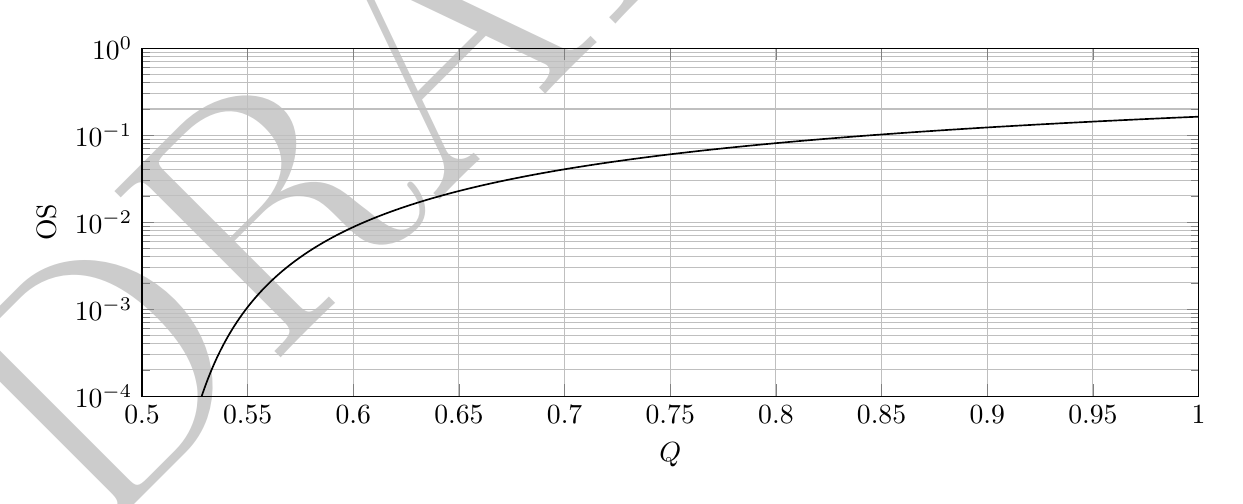
\begin{tikzpicture}
    \begin{axis}[ xlabel=$Q$ 
                , xmin=0.5
                , xmax=1
                , ymin=0.0001
                , ymax=1
                , ylabel=$\mathrm{OS}$
                , grid=both
                , xtick={0.5,0.55,...,1}
                , ymode=log
                , width=15cm
                , height=6cm
                ]
        \addplot [  draw=black
                  , domain=0.501:1
                  , samples=501
                  , smooth
                  , semithick
                  ]
                  ({x},{e^(-pi/sqrt(4*x^2-1))});
    \end{axis}              
  \end{tikzpicture}
  \caption{Overshoot $\mathrm{OS}$ vs. quality $Q\in\left(0.5,1\right]$}
  \label{fig:os2}
\end{figure}


\begin{table}[H]
\centering
\caption{Overshoot $\mathrm{OS}$}
\begin{tabular}{ccc}
\toprule
$Q$                      & $\zeta$                   & $\mathrm{OS}$ in \si{\percent}  \\ \midrule
$\nicefrac{1}{\sqrt{3}}$ & $\nicefrac{\sqrt{3}}{2}$  & 0.43                            \\ \midrule
0.581                    & 0.861                     & 0.5                             \\ \midrule
0.605                    & 0.826                     & 1                               \\ \midrule
0.641                    & 0.78                      & 2                               \\ \midrule
0.657                    & 0.761                     & 2.5                             \\ \midrule
0.671                    & 0.745                     & 3                               \\ \midrule
0.699                    & 0.715                     & 4                               \\ \midrule
$\nicefrac{1}{\sqrt{2}}$ & $\nicefrac{1}{\sqrt{2}}$  & 4.32                            \\ \midrule
0.725                    & 0.69                      & 5                               \\ \midrule
0.786                    & 0.636                     & 7.5                             \\ \midrule
0.845                    & 0.592                     & 10                              \\ \midrule
0.85                     & 0.588                     & 10.18                           \\ \midrule
1                        & 0.5                       & 16.3                            \\ \midrule
1.097                    & 0.456                     & 20                              \\ \midrule
1.239                    & 0.404                     & 25                              \\ \midrule
1.397                    & 0.358                     & 30                              \\ \midrule
$\sqrt{2}$               & 0.354                     & 30.5                            \\ \midrule
1.786                    & 0.28                      & 40                              \\ \midrule
2                        & 0.25                      & 44.43                           \\ \midrule
2.32                     & 0.216                     & 50                              \\ \midrule
3.115                    & 0.161                     & 60                              \\ \midrule
4.432                    & 0.113                     & 70                              \\ \midrule
5                        & 0.1                       & 72.92                           \\ \midrule
5.483                    & 0.091                     & 75                              \\ \toprule
\end{tabular}
\label{tab:os}
\end{table}


\subsection{Delay- and Rise Time}
Two relevant metrics of the step response is the 
\textit{delay time} $t_{\mathrm{d}}$
and the \textit{rising time} $t_{\mathrm{r}}$.
The delay time is the time it takes for the output signal 
$y(t)$ to get from 0 to \SI{50}{\percent} (Fig.~\ref{fig:td-def}).
\begin{figure}[H]
  \centering
  \begin{subfigure}[b]{0.475\textwidth}
    \centering
    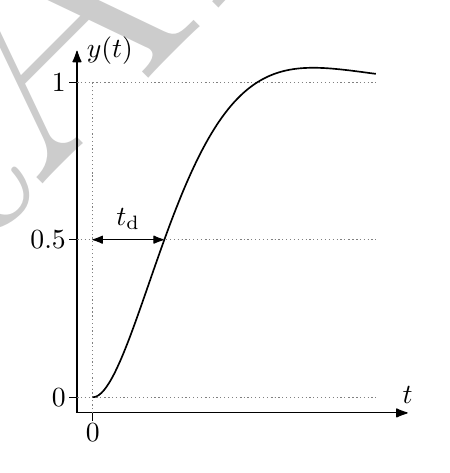
\begin{tikzpicture}[scale=4]
      \draw[{Latex[round,scale=1.0,round]}-{Latex[round,scale=1.0,round]}] 
        (-0.05,1.1) -- (-0.05,-0.05) -- (1,-0.05);

      \node[anchor=south] at  (1,-0.05) {$t$}; 
      \node[anchor=west]  at  (-0.05,1.1) {$y(t)$}; 

      \draw (-0.05,0.0) --++ (-0.025,0) node[anchor=east, inner sep=1pt] {0};
      \draw (-0.05,0.5) --++ (-0.025,0) node[anchor=east, inner sep=1pt] {0.5};
      \draw (-0.05,1.0) --++ (-0.025,0) node[anchor=east, inner sep=1pt] {1};
      \draw (0.0,-0.05) --++ (0,-0.025) node[anchor=north, inner sep=1pt] {0};

      \draw[densely dotted,gray] plot[smooth,domain=-0.05:0.9, samples=2] 
        ({\x},{1});
      \draw[densely dotted,gray] plot[smooth,domain=-0.05:0.9, samples=2] 
        ({\x},{0});
      \draw[densely dotted,gray] plot[smooth,domain=-0.05:0.9, samples=2] 
        ({\x},{0.5});
      \draw[densely dotted,gray] plot[smooth,domain=-0.05:1.0, samples=2] 
        ({0},{\x});

      \draw[semithick] plot[smooth,domain=0:0.9, samples=101] 
        ({\x},{1-e^(-0.7*2*pi*\x)*sin(360*sqrt(1-0.7^2)*\x+acos(0.7))/sin(acos(0.7))});

      \draw[{Latex[round,scale=0.9,round]}-{Latex[round,scale=0.9,round]}] 
        (0,0.5) -- (0.225,0.5) node[above,midway] {$t_{\mathrm{d}}$};
    \end{tikzpicture}
    \caption{Definition of the delay time $t_{\mathrm{d}}$}
    \label{fig:td-def}
  \end{subfigure}%
  \hfill
  \begin{subfigure}[b]{0.475\textwidth}
    \centering
    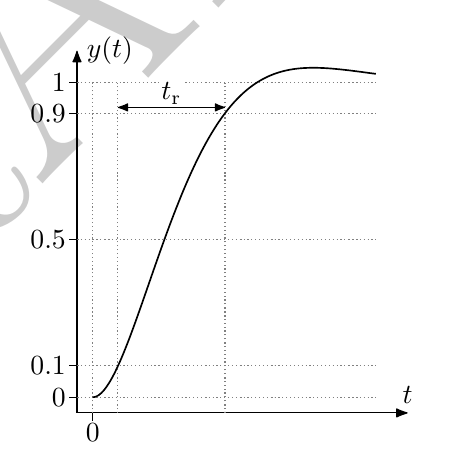
\begin{tikzpicture}[scale=4]
      \draw[{Latex[round,scale=1.0,round]}-{Latex[round,scale=1.0,round]}] 
        (-0.05,1.1) -- (-0.05,-0.05) -- (1,-0.05);

      \node[anchor=south] at  (1,-0.05) {$t$}; 
      \node[anchor=west]  at  (-0.05,1.1) {$y(t)$}; 

      \draw (-0.05,0.0) --++ (-0.025,0) node[anchor=east, inner sep=1pt] {0};
      \draw (-0.05,0.1) --++ (-0.025,0) node[anchor=east, inner sep=1pt] {0.1};
      \draw (-0.05,0.5) --++ (-0.025,0) node[anchor=east, inner sep=1pt] {0.5};
      \draw (-0.05,0.9) --++ (-0.025,0) node[anchor=east, inner sep=1pt] {0.9};
      \draw (-0.05,1.0) --++ (-0.025,0) node[anchor=east, inner sep=1pt] {1};
      \draw (0.0,-0.05) --++ (0,-0.025) node[anchor=north, inner sep=1pt] {0};

      \draw[densely dotted,gray] plot[smooth,domain=-0.05:0.9, samples=2] 
        ({\x},{1});
      \draw[densely dotted,gray] plot[smooth,domain=-0.05:0.9, samples=2] 
        ({\x},{0});
      \draw[densely dotted,gray] plot[smooth,domain=-0.05:0.9, samples=2] 
        ({\x},{0.5});
      \draw[densely dotted,gray] plot[smooth,domain=-0.05:0.9, samples=2] 
        ({\x},{0.1});     
      \draw[densely dotted,gray] plot[smooth,domain=-0.05:0.9, samples=2] 
        ({\x},{0.9});   
      \draw[densely dotted,gray] plot[smooth,domain=-0.05:1.0, samples=2] 
        ({0},{\x});
      \draw[densely dotted,gray] plot[smooth,domain=-0.05:1.0, samples=2] 
        ({0.08},{\x});
      \draw[densely dotted,gray] plot[smooth,domain=-0.05:1.0, samples=2] 
        ({0.42},{\x});

      \draw[semithick] plot[smooth,domain=0:0.9, samples=101] 
        ({\x},{1-e^(-0.7*2*pi*\x)*sin(360*sqrt(1-0.7^2)*\x+acos(0.7))/sin(acos(0.7))});

      \draw[{Latex[round,scale=0.9,round]}-{Latex[round,scale=0.9,round]}] 
        (0.08,0.92) -- (0.42,0.92) node[above,midway,fill=white,inner sep=1pt] {$t_{\mathrm{r}}$};
    \end{tikzpicture}
    \caption{Definition of the rising time $t_{\mathrm{r}}$}
    \label{fig:tr-def}
  \end{subfigure}
  \caption{Definition of the delay time $t_{\mathrm{d}}$ and the rising time $t_{\mathrm{r}}$}
  \label{fig:td-tr-def}
\end{figure}
The rising time $t_{\mathrm{r}}$ is the time it takes for the output signal 
$y(t)$ to get from \SI{10}{\percent} to \SI{90}{\percent} (Fig.~\ref{fig:tr-def}).
We may also use \SI{20}{\percent}-\SI{80}{\percent} or
\SI{30}{\percent}-\SI{70}{\percent} as relevant ranges for definition of
the rising time.

\medskip

The delay- and rising time for different $Q$ is shown in 
Fig. \ref{fig:tdtr}.
Tab. \ref{tab:tdtr} details some relevant values.

\begin{figure}[H]
  \centering
  \begin{tikzpicture}
    \begin{axis}[ xlabel=$Q$ 
                , xmin=0.1
                , xmax=10
                , ymin=0.1
                , ymax=5
                , ylabel=$\nicefrac{t}{T_{0}}$
                , grid=both
                , width=16cm
                , height=8cm
                , ymode=log
                , xmode=log
                ]

    \addplot[ semithick
            ]
            table
            [ x=Q
            , y=td
            , col sep=comma
            ] {delay-rising.csv};    
    \node[fill=white,inner sep=0.5pt,anchor=east] (td) 
      at (0.15,0.3) {$\nicefrac{t_{\mathrm{d}}}{T_{0}}$};
    \draw[thin,gray] (td.north) -- (axis cs:0.1567,0.7122);

    \addplot[ semithick
            ]
            table
            [ x=Q
            , y=tr1090
            , col sep=comma
            ] {delay-rising.csv}; 
    \node[fill=white,inner sep=0.5pt,anchor=west] (tr1090) 
      at (0.25,3.5) {$\nicefrac{t_{\mathrm{r}}}{T_{0}}$(\SI{10}{\percent}-\SI{90}{\percent})};
    \draw[thin,gray] (tr1090.west) -- (axis cs:0.2013,1.6653);

    \addplot[ semithick
            ]
            table
            [ x=Q
            , y=tr2080
            , col sep=comma
            ] {delay-rising.csv}; 
    \node[fill=white,inner sep=0.5pt,anchor=west] (tr2080) 
      at (0.5,2) {$\nicefrac{t_{\mathrm{r}}}{T_{0}}$(\SI{20}{\percent}-\SI{80}{\percent})};
    \draw[thin,gray] (tr2080.west) -- (axis cs:0.3495,0.5511);

    \addplot[ semithick
            ]
            table
            [ x=Q
            , y=tr3070
            , col sep=comma
            ] {delay-rising.csv}; 
    \node[fill=white,inner sep=0.5pt] (tr3070) 
      at (0.28,0.13) {$\nicefrac{t_{\mathrm{r}}}{T_{0}}$(\SI{30}{\percent}-\SI{70}{\percent})};
    \draw[thin,gray] (tr3070.east) -- (axis cs:0.6054,0.1735);

    \end{axis}              
  \end{tikzpicture}
  \caption{Delay time $t_{\mathrm{d}}$ and the rising time $t_{\mathrm{r}}$ vs. $Q$}
  \label{tab:tdtr}
\end{figure}

\begin{table}[H]
\centering
\caption{Delay time $t_{\mathrm{d}}$ and rising time $t_{\mathrm{r}}$}
\begin{tabular}{cccccc}
\toprule
$Q$                      & $\zeta$                   & $\nicefrac{t_{\mathrm{d}}}{T_0}$ & $\nicefrac{t_{\mathrm{r}}}{T_0}$ (\SI{10}{\percent}-\SI{90}{\percent}) & $\nicefrac{t_{\mathrm{r}}}{T_0}$ (\SI{20}{\percent}-\SI{80}{\percent}) & $\nicefrac{t_{\mathrm{r}}}{T_0}$ (\SI{30}{\percent}-\SI{70}{\percent}) \\ \midrule
0.1                      & 5                         & 1.108                            & 3.461                                                                  & 2.184                                                                  & 1.335                                                                  \\
0.25                     & 2                         & 0.456                            & 1.31                                                                   & 0.824                                                                  & 0.503                                                                  \\ 
0.5                      & 1                         & 0.267                            & 0.535                                                                  & 0.345                                                                  & 0.214                                                                  \\ 
$\nicefrac{1}{\sqrt{3}}$ & $\nicefrac{\sqrt{3}}{2}$  & 0.248                            & 0.435                                                                  & 0.29                                                                   & 0.182                                                                  \\ 
$\nicefrac{1}{\sqrt{2}}$ & $\nicefrac{1}{\sqrt{2}}$  & 0.228                            & 0.342                                                                  & 0.237                                                                  & 0.151                                                                  \\ 
0.85                     & 0.588                     & 0.215                            & 0.291                                                                  & 0.205                                                                  & 0.132                                                                  \\ 
1                        & 0.5                       & 0.206                            & 0.261                                                                  & 0.185                                                                  & 0.12                                                                   \\ 
$\sqrt{2}$               & 0.354                     & 0.193                            & 0.222                                                                  & 0.159                                                                  & 0.103                                                                  \\ 
2                        & 0.25                      & 0.184                            & 0.2                                                                    & 0.143                                                                  & 0.093                                                                  \\ 
5                        & 0.1                       & 0.173                            & 0.176                                                                  & 0.125                                                                  & 0.081                                                                  \\ \toprule
\end{tabular}
\label{tab:char-td-tr}
\end{table}

\subsection{Settling Time}

\begin{figure}[H]
  \centering
  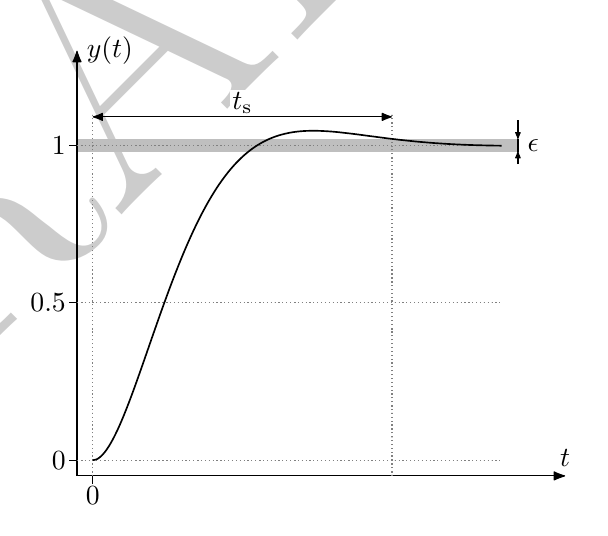
\begin{tikzpicture}[scale=4]
    \fill[lightgray] (-0.05,0.98) rectangle (1.35,1.02);

    \draw[{Latex[round,scale=1.0,round]}-{Latex[round,scale=1.0,round]}] 
      (-0.05,1.3) -- (-0.05,-0.05) -- (1.5,-0.05);

    \node[anchor=south] at  (1.5,-0.05) {$t$}; 
    \node[anchor=west]  at  (-0.05,1.3) {$y(t)$}; 

    \draw (-0.05,0.0) --++ (-0.025,0) node[anchor=east, inner sep=1pt] {0};
    \draw (-0.05,0.5) --++ (-0.025,0) node[anchor=east, inner sep=1pt] {0.5};
    \draw (-0.05,1.0) --++ (-0.025,0) node[anchor=east, inner sep=1pt] {1};
    \draw (0.0,-0.05) --++ (0,-0.025) node[anchor=north, inner sep=1pt] {0};

    \draw[densely dotted,gray] plot[smooth,domain=-0.05:1.3, samples=2] 
      ({\x},{1});
    \draw[densely dotted,gray] plot[smooth,domain=-0.05:1.3, samples=2] 
      ({\x},{0});
    \draw[densely dotted,gray] plot[smooth,domain=-0.05:1.3, samples=2] 
      ({\x},{0.5});
    \draw[densely dotted,gray] plot[smooth,domain=-0.05:1.1, samples=2] 
      ({0},{\x});
    \draw[densely dotted,gray] plot[smooth,domain=-0.05:1.1, samples=2] 
      ({0.95},{\x});
    \draw[{Latex[round,scale=0.9,round]}-{Latex[round,scale=0.9,round]}] 
      (0.0,1.09) -- (0.95,1.09) node[above,midway,fill=white,inner sep=1pt] {$t_{\mathrm{s}}$};

    \draw[semithick] plot[smooth,domain=0:1.3, samples=101] 
      ({\x},{1-e^(-0.7*2*pi*\x)*sin(360*sqrt(1-0.7^2)*\x+acos(0.7))/sin(acos(0.7))});

    \draw[-{Latex[round,scale=0.65,round]}]  (1.35,1.08) -- (1.35,1.02);
    \draw[-{Latex[round,scale=0.65,round]}]  (1.35,0.94) -- (1.35,0.98);
    \draw[]  (1.35,1.02) -- (1.35,0.98);
    \node[anchor=west] at (1.35,1) {$\epsilon$};

  \end{tikzpicture}
  \caption{Definition of the settling time $t_{\mathrm{s}}$}
  \label{fig:ts-def}
\end{figure}

\begin{figure}[H]
  \centering
  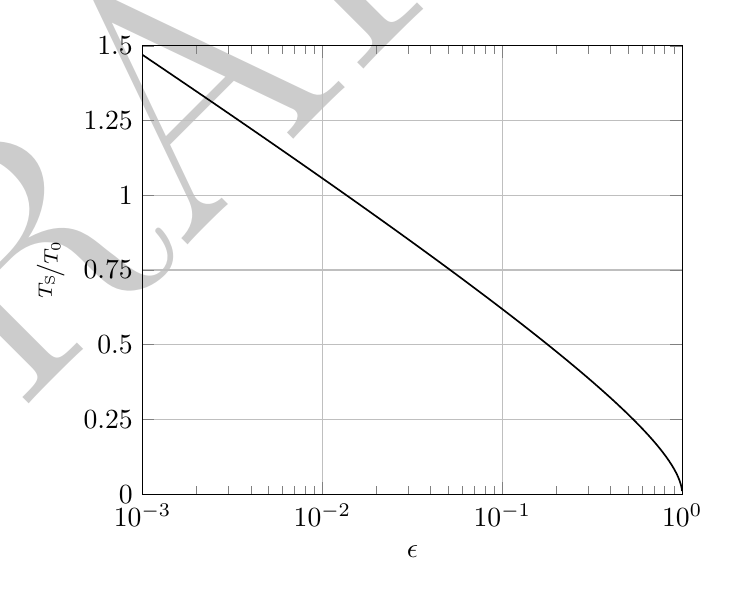
\begin{tikzpicture}
    \begin{axis}[ xlabel=$\epsilon$
                , xmin=1e-3
                , xmax=1
                , ymin=0
                , ymax=1.5
                , ylabel=$\nicefrac{T_{\mathrm{S}}}{T_{\mathrm{0}}}$
                , grid=major
                , ytick={0,0.25,...,1.5}
                , xmode=log
                ]
        \addplot [  draw=black
                  , domain=0.01:1.5
                  , samples=501
                  , smooth
                  , semithick
                  ]
                  ({e^(-2*pi*x)*(1+2*pi*x)},{x});
    \end{axis}              
  \end{tikzpicture}
  \caption{Relative settling time $\nicefrac{T_{\mathrm{S}}}{T_{\mathrm{0}}}$
    vs. deviation $\epsilon$ from final value in the critically damped case}
  \label{fig:settling-crit-damped}
\end{figure}


\section{Examples}\label{sec:examples}

\subsection{Butterworth}\label{subsec:examples:butterworth}

\begin{equation}
\underline{F}_{\mathrm{BW,2}} = \frac{\underline{Y}(s)}{\underline{X}(s)} 
                 = \frac{\omega_0^2}{s^2 + \sqrt{2} \omega_0 s + \omega_0^2 }
\end{equation}



\begin{equation}
Q_{\mathrm{BW,2}}(s) = \frac{1}{\sqrt{2}}
\end{equation}

\begin{equation}
\left|\underline{F}_{\mathrm{BW,2}}\right|
                 = \frac{1}{\sqrt{1+\left(\frac{\omega}{\omega_0}\right)^4}}
\end{equation}

\subsection{Bessel}
tbd
\begin{equation}
Q_{\mathrm{BS,2}}(s) = \frac{1}{\sqrt{3}}
\end{equation}
\subsection{Series RLC}

\begin{figure}[H]
  \centering
  \begin{circuitikz}
    \RlcSeriesSchematicA
  \end{circuitikz}
  \caption{Schematic of series RLC resonator}
  \label{fig:series-res}
\end{figure}

\begin{equation}\label{eq:rlc-series:fs}
\underline{F}(s) = \frac{\underline{V}_{\mathrm{O}}(s)}{\underline{V}_{\mathrm{I}}(s)} 
                 = \frac{\frac{1}{sC}}{R+sL+\frac{1}{sC}}
                 = \frac{1}{1 + sRC+s^2LC}
                 = \frac{\frac{1}{LC}}{s^2+s \frac{R}{L} + \frac{1}{LC}}                 
\end{equation}

A coefficient comparison between \eqref{eq:rlc-series:fs} and \eqref{eq:fs}
results in 
\begin{equation}
\omega_0 = \frac{1}{\sqrt{LC}}
\end{equation}
and
\begin{equation}
Q_{\mathrm{S}} = \frac{L}{R} \omega_0 = \frac{1}{R} \sqrt{\frac{L}{C}}.
\end{equation}

The quality is the ratio between the reactance of L or C and the resistance, 
i.e.
\begin{equation}
Q = \frac{X}{R} = \frac{1}{\omega_0 R C} = \frac{\omega_0 L}{R}.
\end{equation}

\subsection{Parallel RLC}
\begin{equation}
\underline{F}(s) = \frac{\underline{I}_{\mathrm{O}}(s)}{\underline{I}_{\mathrm{I}}(s)} 
                 = \frac{\frac{1}{sL}}{\frac{1}{R}+sC+\frac{1}{sL}}
                 = \frac{1}{1 + \frac{sL}{R}+s^2LC}
                 = \frac{\frac{1}{LC}}{s^2+s \frac{1}{RC} + \frac{1}{LC}}                 
\end{equation}

\begin{equation}
Q_{\mathrm{P}} = R \sqrt{\frac{C}{L}}.
\end{equation}

\printbibliography
\end{document}